\documentclass[tikz,border=8pt]{standalone}
% Shared look for every TikZ diagram. Load with \input{../../tools/tikz-style.tex}
\usepackage[T1]{fontenc}
\usepackage{lmodern}
\renewcommand{\sfdefault}{lmr}  % diagrams use the same serif as the text
\usetikzlibrary{arrows.meta, positioning, shapes.geometric, calc, fit, backgrounds}
\definecolor{cblue}{HTML}{4C78A8}
\definecolor{corange}{HTML}{F58518}
\definecolor{cgreen}{HTML}{54A24B}
\definecolor{cred}{HTML}{E45756}
\definecolor{cpurple}{HTML}{B279A2}
\definecolor{cgrey}{HTML}{6B6B6B}
\tikzset{
  every picture/.style={font=\sffamily, line width=1.2pt},
  box/.style={draw=#1, fill=#1!12, rounded corners=4pt, align=center, inner sep=7pt, minimum height=1.1cm},
  box/.default=cgrey,
  arrow/.style={-{Stealth[length=3mm]}, draw=cgrey, line width=1.4pt},
  title/.style={font=\sffamily\bfseries\Large},
  note/.style={font=\sffamily\small, text=cgrey, align=center},
}
\AtBeginDocument{\hyphenpenalty=10000 \exhyphenpenalty=10000}

\begin{document}
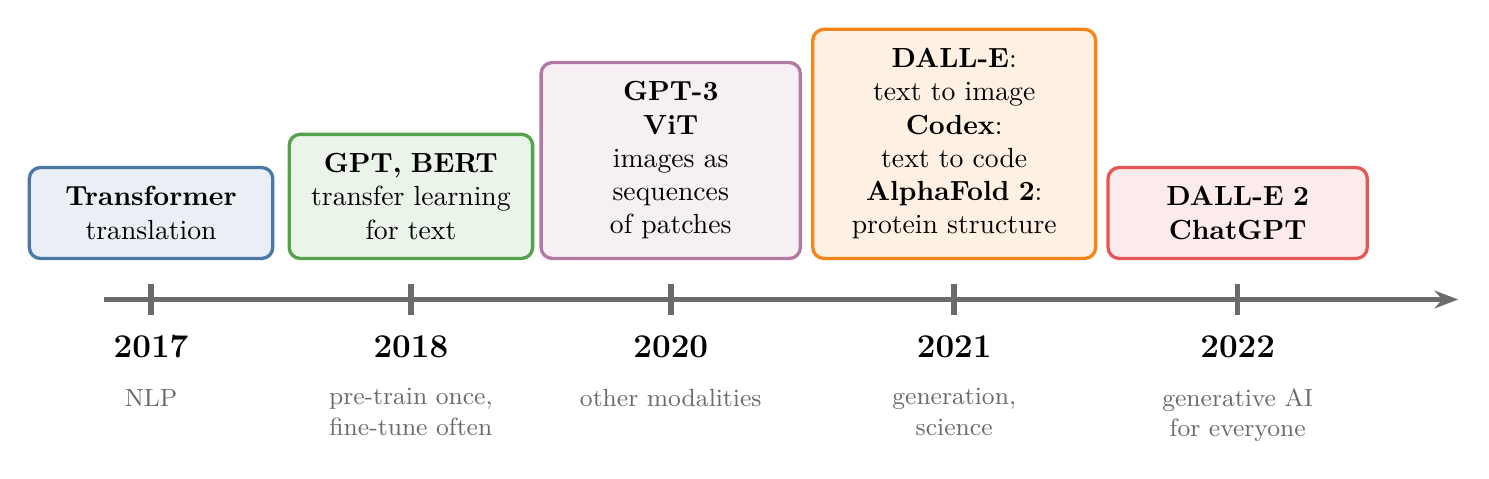
\begin{tikzpicture}[every node/.append style={font=\sffamily}]
  \draw[arrow, line width=2pt] (0,0) -- (17.2,0);
  \foreach \x/\y in {0/2017, 3.3/2018, 6.6/2020, 10.2/2021, 13.8/2022} {
    \draw[cgrey, line width=2pt] (\x+0.6,0.2) -- (\x+0.6,-0.2);
    \node[font=\sffamily\bfseries\large] at (\x+0.6,-0.6) {\y};
  }
  \node[box=cblue, text width=2.6cm, anchor=south] at (0.6,0.5) {\textbf{Transformer}\\translation};
  \node[box=cgreen, text width=2.6cm, anchor=south] at (3.9,0.5) {\textbf{GPT, BERT}\\transfer learning\\for text};
  \node[box=cpurple, text width=2.8cm, anchor=south] at (7.2,0.5) {\textbf{GPT-3}\\\textbf{ViT}\\images as\\sequences of patches};
  \node[box=corange, text width=3.1cm, anchor=south] at (10.8,0.5) {\textbf{DALL-E}: text to image\\\textbf{Codex}: text to code\\\textbf{AlphaFold 2}:\\protein structure};
  \node[box=cred, text width=2.8cm, anchor=south] at (14.4,0.5) {\textbf{DALL-E 2}\\\textbf{ChatGPT}};
  \node[note, below=1.0cm of {(0.6,0)}, text width=2.6cm] {NLP};
  \node[note, below=1.0cm of {(3.9,0)}, text width=2.6cm] {pre-train once,\\fine-tune often};
  \node[note, below=1.0cm of {(7.2,0)}, text width=2.8cm] {other modalities};
  \node[note, below=1.0cm of {(10.8,0)}, text width=3.1cm] {generation,\\science};
  \node[note, below=1.0cm of {(14.4,0)}, text width=2.8cm] {generative AI\\for everyone};
\end{tikzpicture}
\end{document}
